
\section{Úlohy}
Cieľom projektu je vytvoriť autonómny systém na riadenie dronu s využitím ROS, ktorý bude schopný autonómne navigovať v prostredí s prekážkami. Projekt zahŕňa načítanie máp, plánovanie trajektórie a kontrolu pozície dronu na základe zadaných bodov a aktuálnej polohy dronu.
\begin{enumerate}
    \item \textbf{Spracovanie máp}
    \begin{itemize}
        \item Implementácia alebo nástroj - načítanie máp - \textbf{povinné}
        \item Implementácia inflácie prekážok - \textbf{povinné}
        \item Implementácia transformácií máp, rotácií atď. - \textbf{ak je potrebné}
    \end{itemize}
    
    \item \textbf{Algoritmus vyhľadávania ciest (Path finding)}
    \begin{itemize}
        \item Implementácia alebo nástroj - algoritmus vyhľadávania ciest - \textbf{povinné}
        \begin{itemize}
            \item Flood fill, RRT, A*...
        \end{itemize}
    \end{itemize}
    
    \item \textbf{Plánovanie trajektórie}
    \begin{itemize}
        \item Implementácia alebo nástroj - optimalizácia trajektórie - \textbf{ak je potrebné}
        \begin{itemize}
            \item Minimálna požiadavka - eliminácia nepotrebných bodov (eliminácia sekvencií horizontálnych, vertikálnych, diagonálnych bodov)
        \end{itemize}
    \end{itemize}
    
    \item \textbf{ROS Uzol pre riadenie dronu}
    \begin{itemize}
        \item Implementácia - načítanie trajektórie - \textbf{povinné}
        \item Implementácia - úlohy/misie - \textbf{povinné}
        \item Implementácia - regulátor polohy - \textbf{povinné}
    \end{itemize}
    
    \item \textbf{Špecifikácia bodu/úlohy/príkazu}
    \begin{itemize}
        \item Implementácia - vzlet a pristátie - \textbf{povinné}
        \item Implementácia - polomer bodu (presnosť regulátora pre daný bod - Hard/Soft) - \textbf{povinné}
        \item Implementácia - riadenie yaw v špecifickom uhle - \textbf{povinné}
    \end{itemize}
    
    \item \textbf{Dokumentácia}
    \begin{itemize}
        \item Analýza každého použitého prístupu - \textbf{povinné}
        \begin{itemize}
            \item Výhody a nevýhody
            \item Vysvetlenie algoritmov alebo implementácií
        \end{itemize}
        \item Celkový diagram riešenia - \textbf{povinné}
        \begin{itemize}
            \item Cesty spracovania dát
            \item Diagram riadenia dronu v ROS
        \end{itemize}
    \end{itemize}
\end{enumerate}

\section{Implementácia}
Implementácia projektu zahŕňa niekoľko kľúčových komponentov vrátane načítania máp, vyhľadávania ciest, optimalizácie trajektórie a vytvárania ROS uzlov pre publikovanie príkazov a sledovanie pozície dronu.

\subsection{Načítanie máp a príprava prekážok}
V projekte sme si vygenerovali názvy súborov máp, ktoré následne načítavame do triedy \texttt{nav\_msgs::msg::OccupancyGrid} z balíčka Navigation2 v ROS2. Po načítaní máp rozširujeme prekážky o 4 pixely, čím zabezpečujeme, že dron bude mať dostatočný odstup od prekážok. 

\subsection{Plánovanie misie a generovanie trajektórie}
Po načítaní máp načítame misiu, ktorá definuje sekvenciu bodov, ktorými musí dron prejsť. Pre generovanie cesty používame algoritmus A*, ktorý je vhodný na nájdenie optimálnej cesty v mriežke. Algoritmus A* kombinuje hľadanie najkratšej vzdialenosti s heuristikou vzdialenosti od cieľa, čo mu umožňuje efektívne nájsť cestu.

Po vygenerovaní cesty eliminujeme nadbytočné body a ponecháme iba zlomové body, čo zvyšuje efektivitu pohybu. Pri pohybe po diagonále navyše odstraňujeme veľký počet bodov. Tento prístup je opísaný nižšie:

\begin{lstlisting}[language=C++, caption={Optimalizácia cesty - odstránenie bodov}]
double dx1 = curr.x - prev.x;
double dy1 = curr.y - prev.y;
double dx2 = next.x - curr.x;
double dy2 = next.y - curr.y;

bool is_approx_straight = !(dx1 * dy2 != dy1 * dx2);
bool is_approx_diagonal = (std::abs(dx1) > tolerance && std::abs(dy1) > tolerance) &&
                          (std::abs(dx1 - dx2) <= tolerance && std::abs(dy1 - dy2) <= tolerance);

if ((!is_approx_diagonal && !is_approx_straight) || 
    (is_approx_straight && (dx1 * dx2 < 0 || dy1 * dy2 < 0))) // Zmena smeru
{
    optimized_path.push_back(path_points[i]);
}
\end{lstlisting}

\subsection{Funkcia pre riadenie pohybu: \texttt{go\_to\_point}}
Vytvorili sme funkciu \texttt{void go\_to\_point(double x, double y, double z, double tolerance)}, ktorá prijíma súradnice cieľa po transponovaní, pretože mapy, simulácia a dron majú rôzne orientácie osí. Parameter \texttt{tolerance} určuje presnosť, s akou má dron doraziť na cieľové súradnice:

\begin{itemize}
    \item Pre \textbf{soft} presnosť je tolerancia 0.1 m.
    \item Pre \textbf{hard} presnosť je tolerancia 0.05 m.
    \item Pre prechodové body je tolerancia 0.25 m.
\end{itemize}

Príkazy pre pohyb dronu publikujeme s frekvenciou 10 Hz. Funkcia zároveň kontroluje, či je aktuálna poloha dronu v rámci požadovanej tolerancie. Ak áno, nastaví sa nový cieľový bod.

\section{Realizácia}

\subsection{Vyhľadávanie ciest}
Na plánovanie trajektórie dronu sa používajú algoritmy na vyhľadávanie ciest, ako sú A* alebo RRT. Tieto algoritmy zabezpečujú, že dron môže navigovať efektívne medzi bodmi v mape, pričom sa vyhýba prekážkam.

\subsubsection{Odstraňovanie bodov}
Po vygenerovaní počiatočnej trajektórie sa vykoná optimalizácia odstránením nadbytočných bodov. Tento proces zahŕňa elimináciu sekvencií bodov, ktoré sú v priamej línii (horizontálnej, vertikálnej alebo diagonálnej), čím sa minimalizuje počet bodov a zvyšuje efektivita pohybu dronu.

\subsection{Vytváranie Publishera}
ROS uzol vytvára Publisher, ktorý publikuje príkazy pre pohyb dronu na základe bodov trajektórie. Publisher je navrhnutý tak, aby odosielal pozíciu dronu na ďalší bod, kým dron nedosiahne cieľovú pozíciu alebo kým nenastane potreba zastaviť publikovanie.

\subsubsection{Kontrola skutočnej polohy pre zastavenie publikovania}
Počas publikovania príkazov na pohyb dronu uzol pravidelne kontroluje skutočnú polohu dronu. Ak dron dosiahne cieľový bod alebo je v blízkosti s dostatočnou presnosťou, publikovanie sa zastaví. Táto kontrola je dôležitá na minimalizovanie počtu odoslaných príkazov a na zabezpečenie presnosti pohybu dronu v rámci požadovaných súradníc.
\subsection{Funkcie pre nastavenie režimu a armovanie dronu}

\subsubsection{\texttt{set\_arm}}
Táto funkcia zaisťuje armovanie dronu. Funkcia vytvára požiadavku na armovanie dronu pomocou ROS služby a čaká na potvrdenie úspešného armovania. Ak armovanie prebehne úspešne, funkcia pokračuje. Ak sa vyskytnú problémy, vygeneruje sa chybové hlásenie. Kód pre funkciu je nasledovný:

\begin{lstlisting}[language=C++, caption={Funkcia pre armovanie dronu}]
void set_arm(){
    auto arm_request = std::make_shared<mavros_msgs::srv::CommandBool::Request>();
    arm_request->value = true;

    while (!arming_client_->wait_for_service(1s))
    {
        if (!rclcpp::ok())
        {
            RCLCPP_ERROR(this->get_logger(), "Interrupted while waiting for the set_mode service. Exiting.");
            return;
        }
        RCLCPP_INFO(this->get_logger(), "Waiting for set_mode service...");
    }

    auto arm_result = arming_client_->async_send_request(arm_request);
    if (rclcpp::spin_until_future_complete(this->get_node_base_interface(), arm_result) == rclcpp::FutureReturnCode::SUCCESS)
    {
        if (arm_result.get()->success)
        {
            RCLCPP_INFO(this->get_logger(), "Drone armed successfully.");
            while (!current_state_.armed)
            {
                rclcpp::spin_some(this->get_node_base_interface());
                std::this_thread::sleep_for(std::chrono::milliseconds(100));
            }
        }
        else
        {
            RCLCPP_ERROR(this->get_logger(), "Failed to arm the drone.");
            return;
        }
    }
}
\end{lstlisting}

\subsubsection{\texttt{set\_mode}}
Funkcia \texttt{set\_mode} nastavuje režim dronu, napríklad na \texttt{GUIDED} alebo \texttt{LAND}. Funkcia posiela požiadavku na nastavenie režimu a overuje, či bol režim úspešne zmenený. Ak je režim nastavený na \texttt{LAND}, funkcia čaká, kým dron nedosiahne výšku 0.15 m pred ukončením. Kód pre funkciu je nasledovný:

\begin{lstlisting}[language=C++, caption={Funkcia pre nastavenie režimu dronu}]
void set_mode(char *mode){
    mavros_msgs::srv::SetMode::Request guided_set_mode_req;
    guided_set_mode_req.custom_mode = mode;
    while (!set_mode_client_->wait_for_service(1s))
    {
        if (!rclcpp::ok())
        {
            RCLCPP_ERROR(this->get_logger(), "Interrupted while waiting for the set_mode service. Exiting.");
            return;
        }
        RCLCPP_INFO(this->get_logger(), "Waiting for set_mode service...");
    }
    auto result = set_mode_client_->async_send_request(std::make_shared<
                        mavros_msgs::srv::SetMode::Request>(guided_set_mode_req));
    if (rclcpp::spin_until_future_complete(this->get_node_base_interface(), result) == rclcpp::FutureReturnCode::SUCCESS)
    {
        RCLCPP_INFO(this->get_logger(), "Drone mode changed to %s", mode);
    }
    else
    {
        RCLCPP_ERROR(this->get_logger(), "Failed to change mode to %s", mode);
        return;
    }
    if(mode == "LAND"){
        while(current_local_pos_.pose.position.z > 0.15){
            rclcpp::spin_some(this->get_node_base_interface());
            std::this_thread::sleep_for(std::chrono::milliseconds(100));
        }
    }
}
\end{lstlisting}
\newpage
\subsection{Node graf}
\begin{figure}[!htpb]
    \centering
    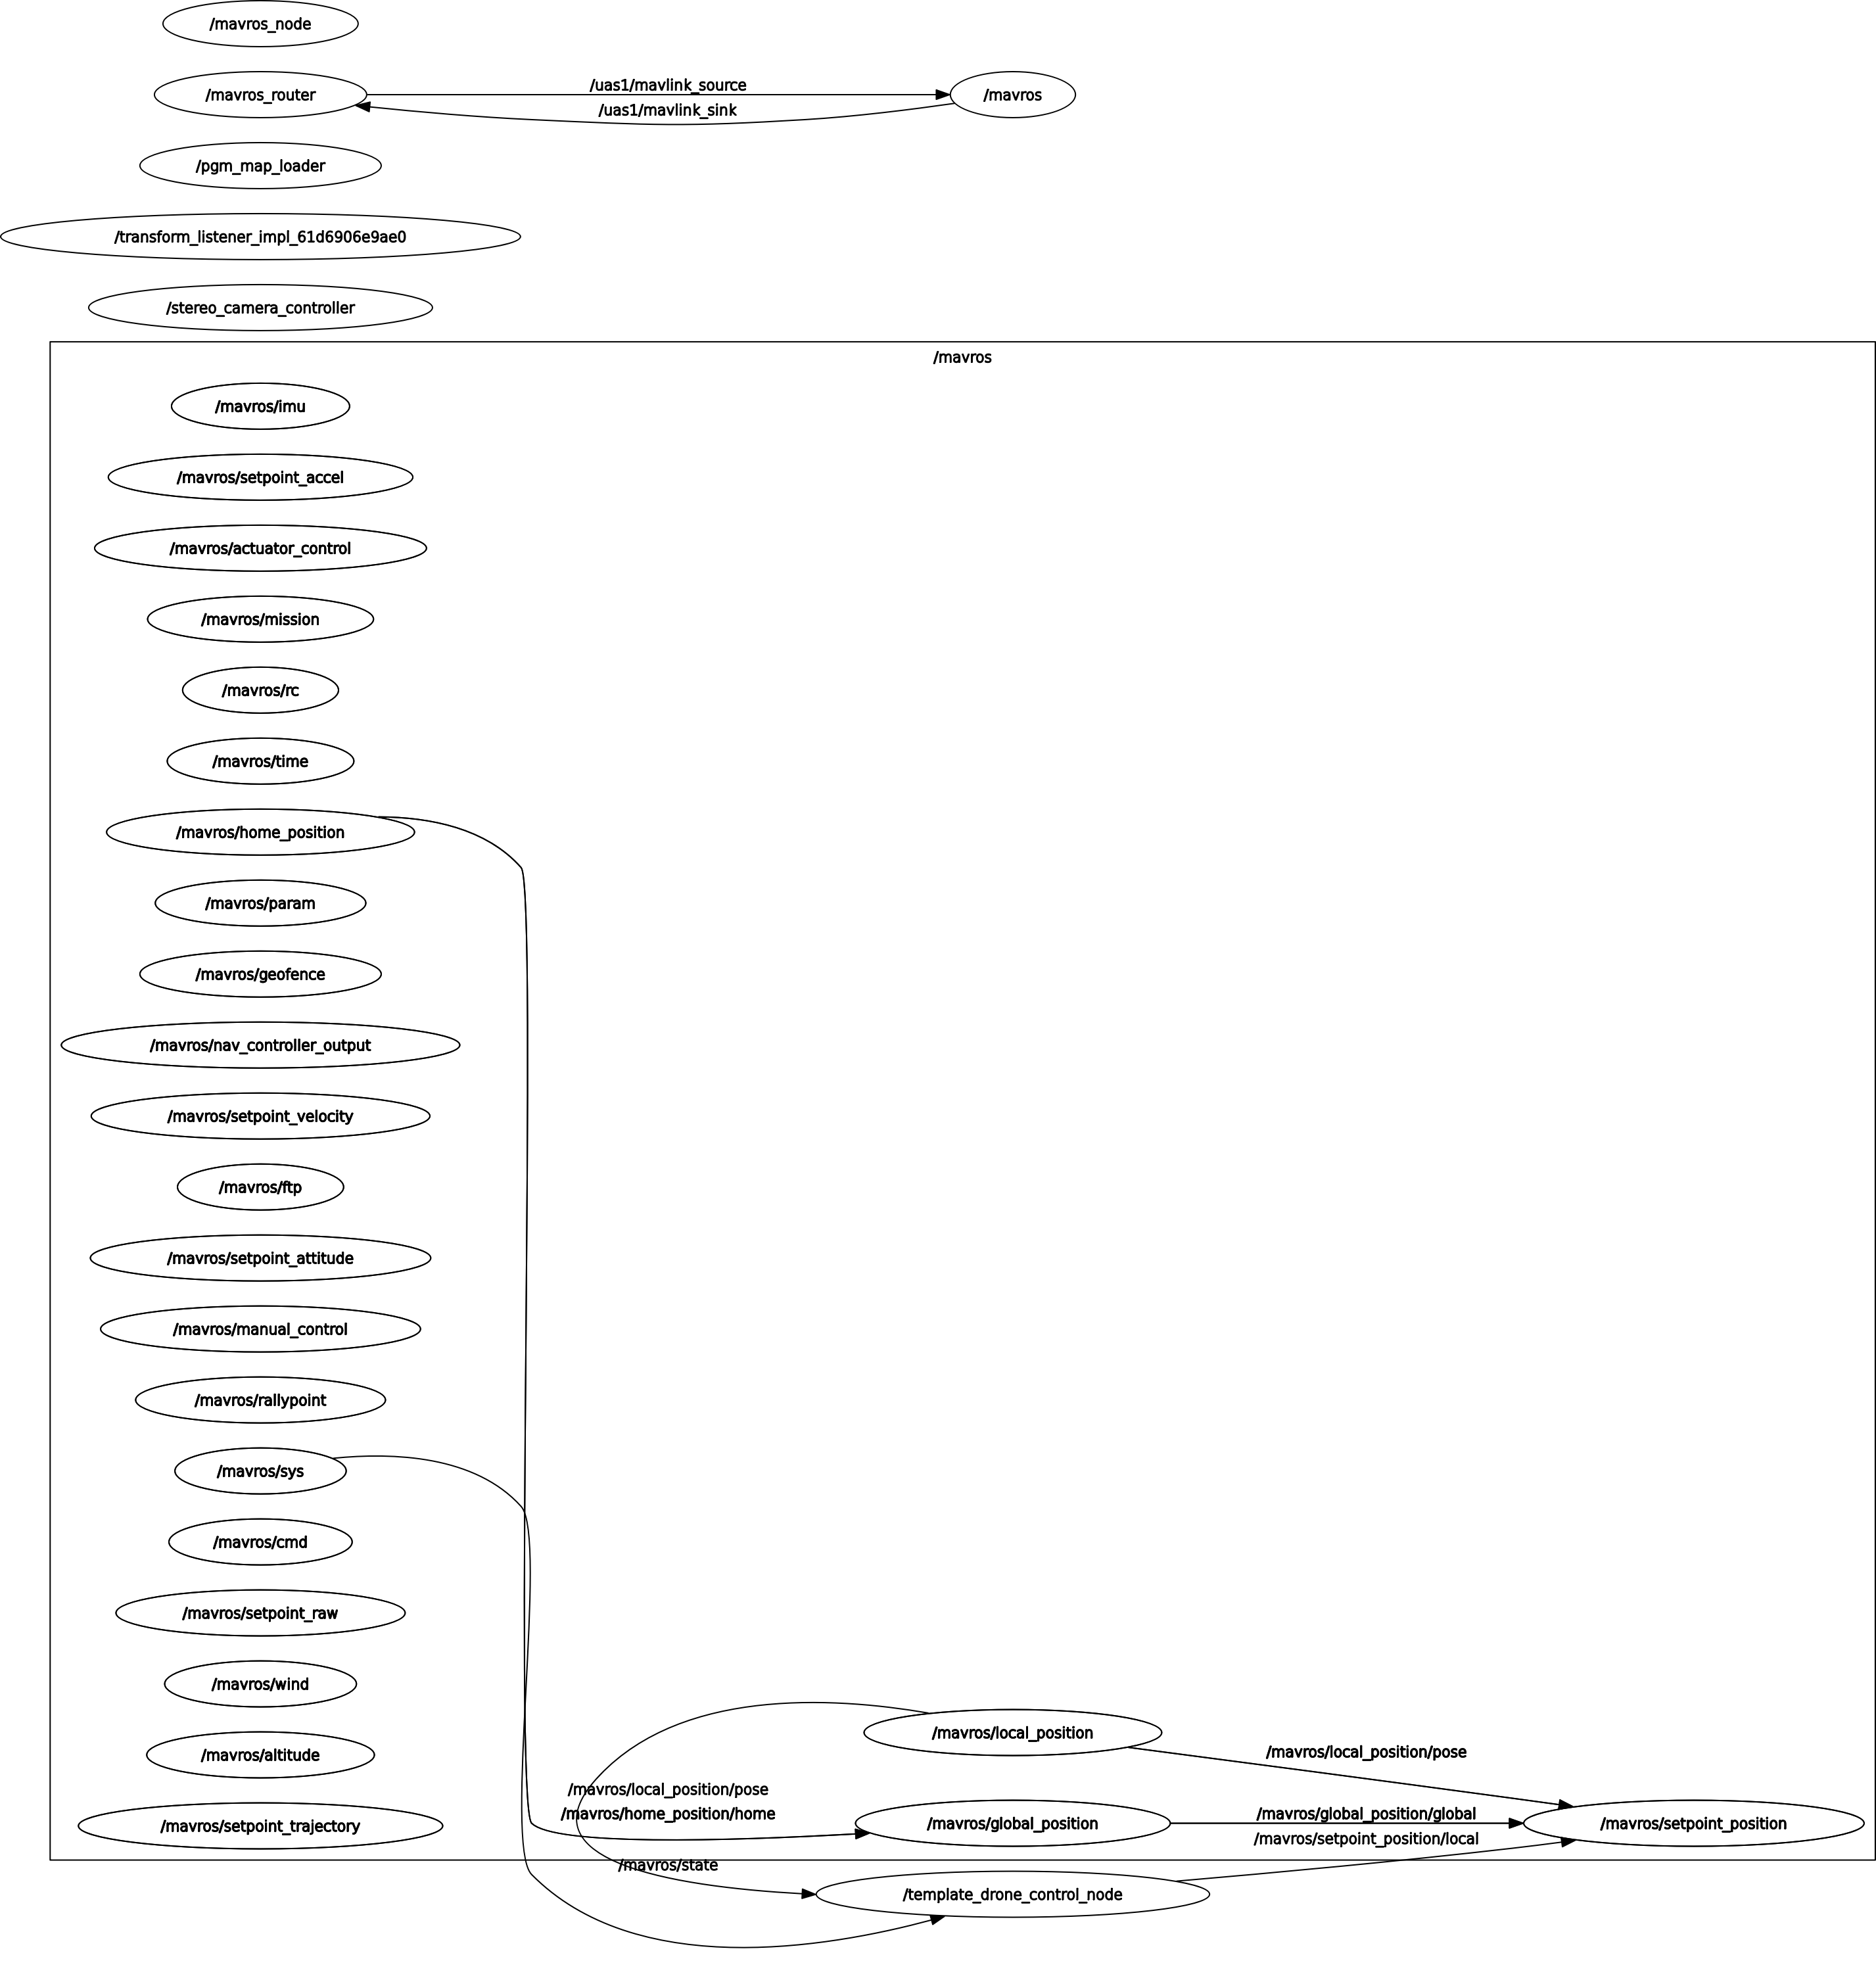
\includegraphics[width=0.8\textwidth]{img/rosgraph.png}
    \caption{Node graf}
    \label{fig:node_graph}
\end{figure}